\scanpage{360}
\hfill EZ 3

Les applications shuffles et A-W sont \uline{assoc}

\figure{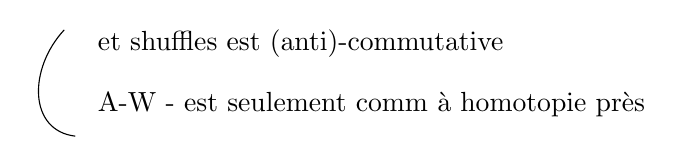
\begin{tikzpicture}
\node[anchor=north west,inner sep=0] (aw) at (0,0) {\begin{tabular}{l}
et \uline{shuffles} est (anti)-commutative\\[10pt]
A-W - est seulement comm à homotopie près
\end{tabular}};
\draw ([xshift=-6pt,yshift=-1pt]aw.north west)
 .. controls ([xshift=-19pt,yshift=-15pt]aw.north west) and ([xshift=-19pt,yshift=-3pt]aw.south west)
 .. ([xshift=-2pt,yshift=-5pt]aw.south west);
\end{tikzpicture}}

On peut exprimer ceci avec des diagrammes d'objet trisimpliciaux

\margin{Ref Illusie\quad\uline{thèse.}}
\diagram{\begin{tikzcd}[column sep=large]
X_{***}\arrow[r,"N_{\unsure{**|12}}"]\arrow[d,"\Delta_{12}"']&X_{\cdot\cdot\cdot}\arrow[r,"\int_{12}"]&X_{\cdot\cdot}\arrow[d,no head,"\int"]\\
X_{**}\arrow[r,"N"]&X_{\cdot\cdot}&X_{\cdot}
\end{tikzcd}}
\figure{\begin{tikzpicture}\draw (0,.15) .. controls (2,0) and (4,-.1) .. (6,-.5);\end{tikzpicture}}
Clair pour $\underbrace{ZX}$.

\deleted{$\unsure{ZX\otimes ZX\otimes ZX|ZX\otimes ZX}\longrightarrow$}
\figure{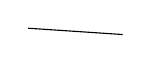
\begin{tikzpicture}\draw (0,0)--(1.2,-.08);\end{tikzpicture}}

L'enoncé de commutativité s'enonce comme suit.
\margin{$X$ ens simpl}

\deleted{$\operatorname{Hom}(ZX\otimes ZX,Z(X\times X))$}
\diagram{\begin{tikzcd}
\operatorname{Hom}^{'}(Z(X\times X)^\sim,\widetilde Z X\otimes\widetilde Z X)\arrow[r]&\mathbb Z
\end{tikzcd}}
\diagram{\begin{tikzcd}[column sep=large]
\text{\margin{$\Sigma_2$ agit sur ce complexe}}\arrow[r,bend right=12]&\operatorname{Hom}(Z(X_0\times X_0)\overset{\sim}{\not\to}ZX_0\otimes ZX_0)\arrow[r]&Z
\end{tikzcd}}
\diagram{\begin{tikzcd}
X\arrow[r]&\mathrm{pt}\arrow[r,draw=none,"{\deleted{\longrightarrow}}" description]&{}
\end{tikzcd}}
\diagram{\begin{tikzcd}
\uline{\operatorname{Hom}(Z(,),\widetilde Z()\otimes\widetilde Z())}\arrow[r]&Z
\end{tikzcd}}

\uline{Theorème} (Dold): ``Ueber Steenrodsche operationen --''

Pour tout $X$, Ce complexe
\[
\left.\begin{gathered}
\operatorname{Hom}^{'}(Z(X\ldots\times X),Z(X)\otimes\ldots\otimes ZX\\
\operatorname{Hom}^{'}(ZX\otimes\ldots\otimes ZX,Z(X\times\ldots\times X)
\end{gathered}\right\}
\]
est une resolution libre de $Z$ dans la cat des $\Sigma_n$-modules
\inserted{pour $X$ variable}

On tronque pour avoir un complexe de chaines
\mspage{361}
